\documentclass{mva2011}
\usepackage{graphicx}
\usepackage{times}
\usepackage{epsfig}
\usepackage{graphicx}
\usepackage{amsmath}
\usepackage{amssymb}
\usepackage{subfigure}
\usepackage{color}
\usepackage[usenames,dvipsnames]{xcolor}
\usepackage{algorithm}
\usepackage{algorithmic}
\usepackage{authblk}
\usepackage{abstract}
\usepackage{comment}
\usepackage{picins}
\usepackage[normalem]{ulem}
\usepackage{url}
 \usepackage{epstopdf}
 \usepackage[section]{placeins}
\renewcommand\Authands{, }

%example for producing articles in MVA2009 format using LaTeX.
%written by Takeshi MASUDA, Electrotechnical Laboratory, Japan in May 1996.
%modified by KAGESAWA Masataka, in May 1998.
%modified by OKAZAKI Shin'ichro, in Feb 2000.
%modified by YASUMOTO Mamoru, in Apr 2002.
%modified by Ken-ichi MAEDA, Dec 2008.
%modified by MASUDA Takeshi, AIST, Oct 2011
%modified by Masaki Onishi, AIST, Oct 2011
%use at your own risk.

\begin{document}
\title{Detection by Motion-based Grouping of Object Parts}

\author[1]{Zhipeng Wang}
\author[2]{Jinshi Cui}
\author[2]{Hongbin Zha}
\author[1]{Masataka Kagesawa}
\author[1]{Shintaro Ono}
\author[1]{Katsushi Ikeuchi}
\affil[1]{Institute of Industrial Science, The University of Tokyo, Japan \authorcr
Email: \{wangzp,kagesawa,onoshin,ki\}@cvl.iis.u-tokyo.ac.jp}
\affil[2]{Key Lab of Machine Perception (Ministry of Education), Peking University, China \authorcr
Email: \{cjs,zha\}@cis.pku.edu.cn}
\twocolumn[
\begin{@twocolumnfalse}
\maketitle
{\normalsize

}

\begin{center}
\emph{\textbf{Keywords: }Object detection, Motion grouping, Common fate}
\end{center}
\emph{}
\\
\end{@twocolumnfalse}
]



\section{Introduction}
% no \IEEEPARstart
% You must have at least 2 lines in the paragraph with the drop letter
% (should never be an issue)

\begin{comment}

Most state-of-the-art detection methods are based on the sliding-window schema~\cite{ac4,ac1} or the Hough transform~\cite{ac2,ac3,ac18}.
The sliding-window methods consider all sub-images by using classifiers to decide whether an object exists or not.
The Hough transform based methods, represented by the ISM~\cite{lb1}, start by detection of object parts, and object hypotheses are given by summing up all the votes voted by the object parts.
\end{comment}



\begin{comment}
Here we focus on techniques from the area of computer vision for detection of pedestrians and bicycle riders under surveillance scenarios.
\end{comment}




















\begin{figure}
\centering
\subfigure[]{
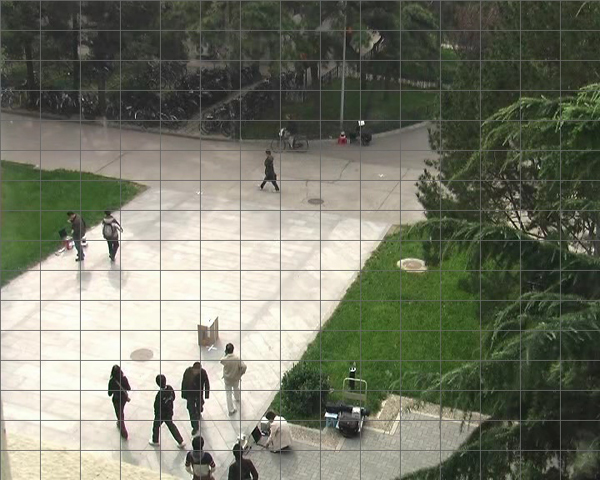
\includegraphics[width=0.22\textwidth,bb=0 0 600 480]{PEssR.jpg}
\label{fig:compa:a}}
\subfigure[]{
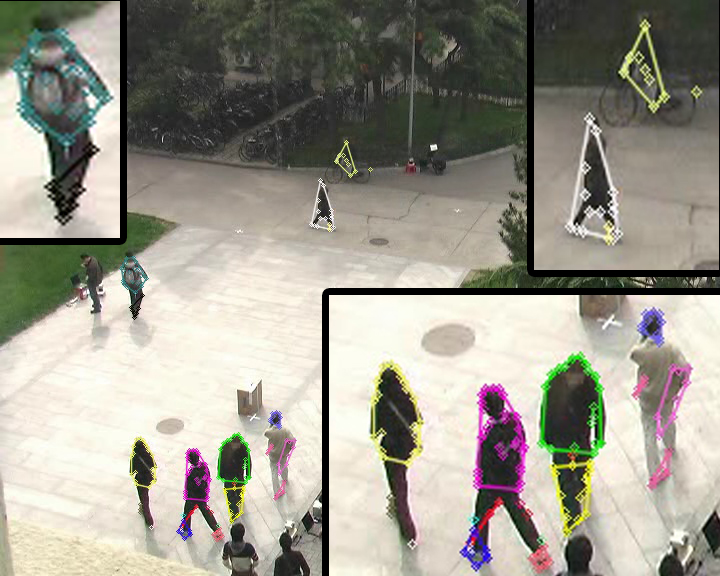
\includegraphics[width=0.22\textwidth,bb=0 0 720 576]{a56.jpg}
\label{fig:compa:b}}
\subfigure[]{
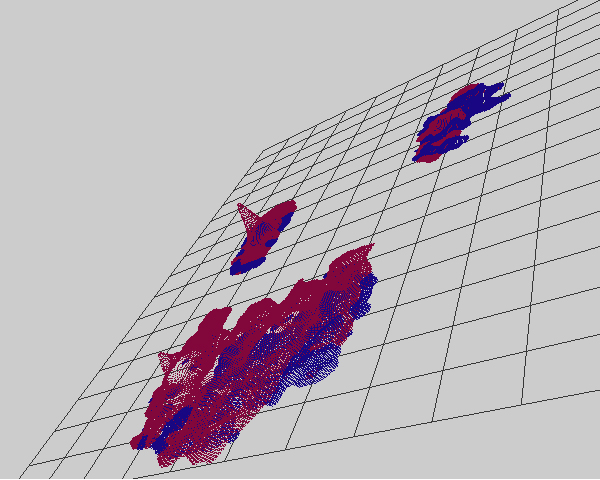
\includegraphics[width=0.22\textwidth,bb=0 0 600 480]{Untitled-6.jpg}
\label{fig:compa:c}}
\subfigure[]{
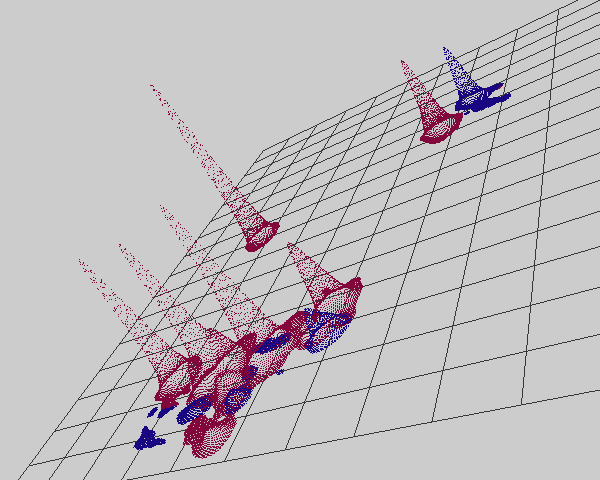
\includegraphics[width=0.22\textwidth,bb=0 0 600 480]{Untitled-4.jpg}
\label{fig:compa:d}
}
\caption{Merit of the proposed method. (a) Original image. (b) Motion   grouping results.  Some parts are enlarged to show details. (c) Original Hough image. (d) Hough image formed using our method. The grids in (c) and (d) correspond to the grids in(a).}
\label{fig:compa}
\end{figure}







\section{Related Work}




\section{Common Fate Hough Transform}




\begin{equation}C({\tilde{\bf{x}}},\tilde{l};{\bf{e}}) = \sum\limits^N_{i=1} {B({\tilde{\bf{x}}},{\tilde{l}};{V_{\bf{e}}^i}) w({V_{\bf{e}}^i})}\:.
\label{eq1}
\end{equation}
Here $B({\tilde{\bf{x}}},{\tilde{l}};{V_{\bf{e}}^i})$ is the blurring function. And $w({V_{\bf{e}}^i})$ is the weight of ${V_{\bf{e}}^i}$.

The idea of the proposed method is that the weight term, $w({V_{\bf{e}}^i})$, is defined by the motion grouping results of all the object parts.

The blurring function is defined as,

\begin{equation}
B(\tilde{\bf{x}},\tilde l;V)
= \left\{ \begin{array}{*{20}{c}}
   0   &\mbox{  if } {l_V} \ne \tilde{l} \mbox{ or } |\tilde{\bf{x}} - {\bf{x}}_V| > d   \\
   G(\tilde{\bf{x}};{{\bf{x}}_V},\sigma) &\mbox{otherwise}
\end{array} \right. \:.
\label{eq2}
\end{equation}


\begin{equation}
\begin{aligned}
C({\tilde{\bf{x}}},\tilde{l}) &=\sum\limits^M_{j=1} C({\tilde{\bf{x}}},\tilde{l};{\bf{e}}_j)w({\bf{e}}_j) \\
&{
\begin{aligned}
=\sum\limits^M_{j=1} \sum\limits^N_{i=1} {B({\tilde{\bf{x}}},{\tilde{l}};{V_{{\bf{e}}_j}^i}) w({V_{{\bf{e}}_j}^i})w({\bf{e}}_j)} \:.
\end{aligned}
}
\end{aligned}
\label{eq3}
\end{equation}



\subsection{Common Fate Weights}




\[
S({V_{{{\bf{e}}_n}}} \to {V_{{{\bf{e}}_m}}})  =  B({\bf{x}}_{V_{{{\bf{e}}_m}}},l_{V_{{{\bf{e}}_m}}};{V_{{{\bf{e}}_n}}})\:,n \ne m\:.
\]


\[
\begin{aligned}
S({{{\bf{e}}_n} \to {V_{{{\bf{e}}_m}}}}) &= C({\bf{x}}_{V_{{{\bf{e}}_m}}},l_{V_{{{\bf{e}}_m}}};{{{\bf{e}}_n}})\\
& {
=\sum\limits^N_{i=1} {S({{V^i_{{{\bf{e}}_n}}} \to {V_{{{\bf{e}}_m}}}})w(V^i_{{\bf{e}}_n})}\:,n \ne m\:.
}
\end{aligned}
\]


\[
\begin{aligned}
S({\bf{g}} \to V_{{\bf{e}}_m})
&= \sum\limits_{{{\bf{e}}_i} \in {\bf{g}}- \{ {{\bf{e}}_m} \} }{C({\bf{x}}_{V_{{{\bf{e}}_i}}},l_{V_{{{\bf{e}}_m}}};{{{\bf{e}}_i}})w({{\bf{e}}_i})}\\
& =\frac 1 M  \sum\limits_{{{\bf{e}}_i} \in {\bf{g}}- \{ {{\bf{e}}_m} \}} {S({{{\bf{e}}_i} \to {V_{{{\bf{e}}_m}}}})} \:.
\end{aligned}
\]


\begin{equation}
\begin{aligned}
{\color{blue}w(}&{\color{blue}{\tilde{V}}_{{\bf{e}}_m})}
= \frac
{S({\bf{g}} \to {{\tilde{V}}_{{\bf{e}}_m}}) + \frac{\Delta } N}
{\sum\limits^N_{i=1}{ S({\bf{g}} \to {V^i_{{{\bf{e}}_m}}})} + \Delta }\\
&
\begin{aligned}
= \frac
{ \sum\limits_{{{\bf{e}}_j} \in {\bf{g}}- \{ {{\bf{e}}_m} \}} {
\sum\limits^N_{k=1} {S({{V^k_{{{\bf{e}}_j}}} \to {{\tilde{V}}_{{{\bf{e}}_m}}}})\color{blue}{w(V^k_{{\bf{e}}_j})}}
}  + \frac{M\Delta } N}
{\sum\limits^N_{i=1}{
\sum\limits_{{{\bf{e}}_j} \in {\bf{g}}- \{ {{\bf{e}}_m} \}} {
\sum\limits^N_{k=1} {S({{V^k_{{{\bf{e}}_j}}} \to {V^i_{{{\bf{e}}_m}}}})\color{blue}{w(V^k_{{\bf{e}}_j})}}
}
} + M\Delta }\:.
\end{aligned}
\end{aligned}
\label{eq4}
\end{equation}


\begin{figure}
\centering
\subfigure[]{
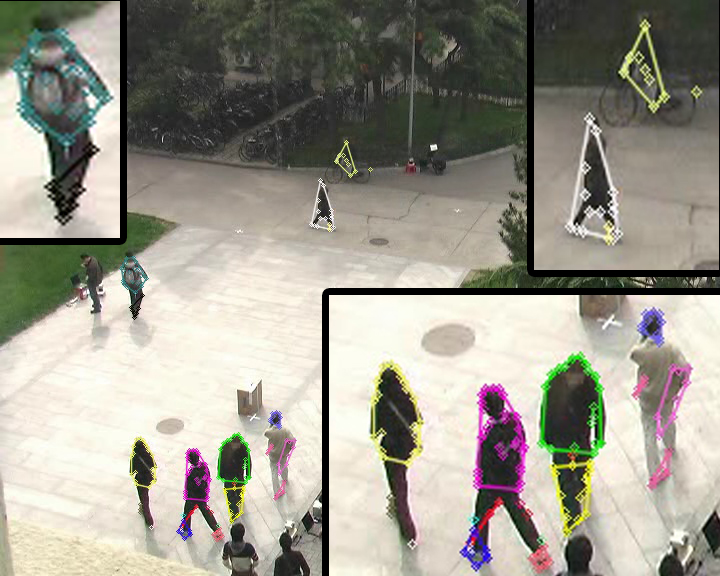
\includegraphics[width=0.22\textwidth,bb=0 0 720 576]{a56.jpg}
\label{fig:compa:a}}
\subfigure[]{
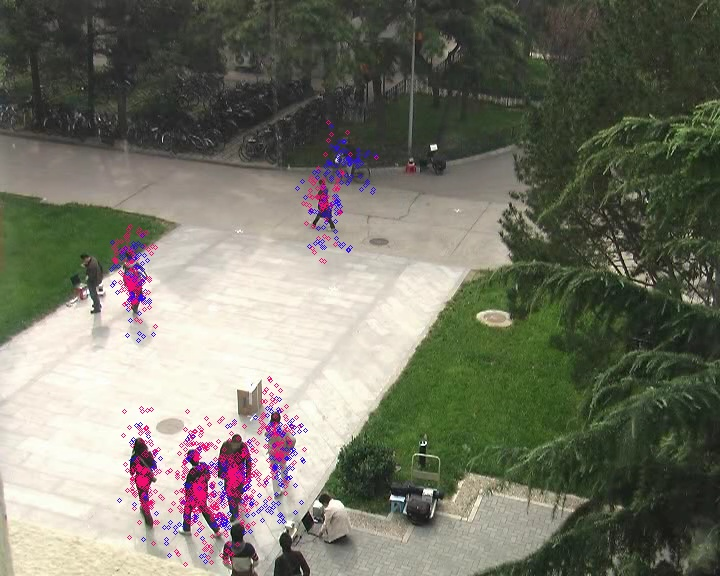
\includegraphics[width=0.22\textwidth,bb=0 0 720 576]{voteimg00056.jpg}
\label{fig:compa:b}}
\subfigure[]{
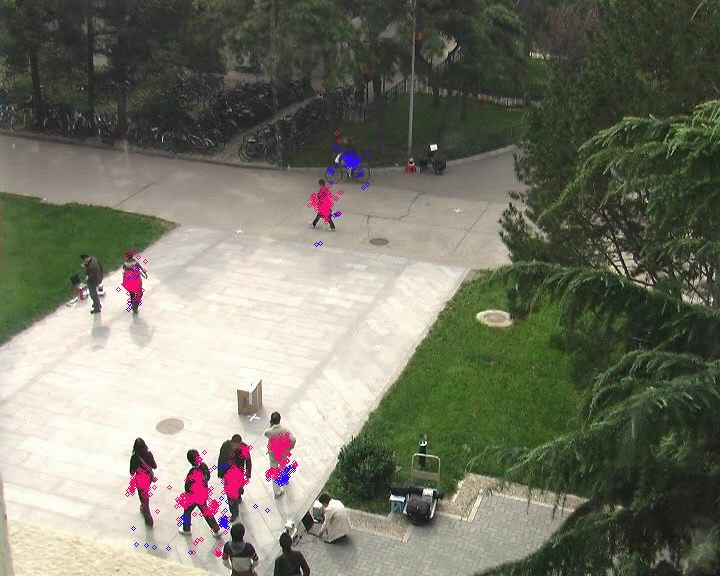
\includegraphics[width=0.22\textwidth,bb=0 0 720 576]{selectVimg00056_9.jpg}
\label{fig:compa:c}}
\subfigure[]{
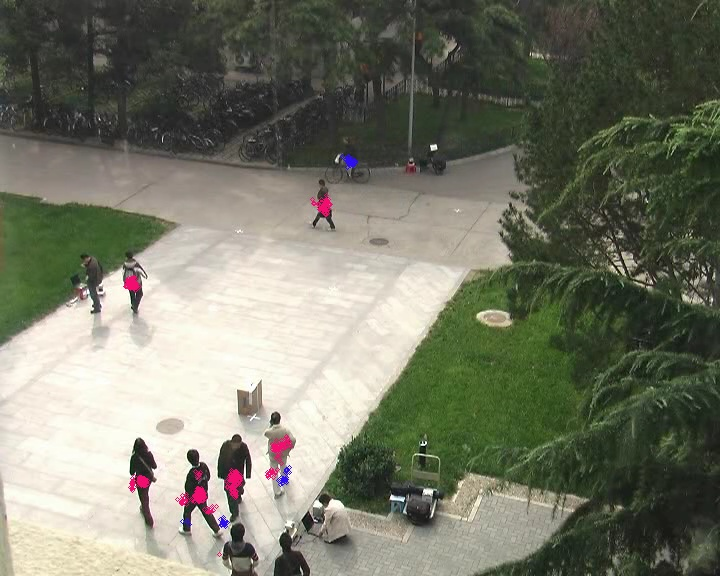
\includegraphics[width=0.22\textwidth,bb=0 0 720 576]{selectedvotesimg00056.jpg}
\label{fig:compa:c}}
\caption{Effect of the proposed weight. (a) Motion groups, different colors mark different motion groups. (b) Voted centers given by the 7 best matched codes. (c) Voted centers with the highest defined weights. (d) Voted centers with weights higher than a threshold.}
\label{fig:compa}
\end{figure}

\subsection{Motion Grouping}


To define the second similarity, the $i$th directional vector of $T$ is firstly defined as, ${\bf{d}}^i_T={\bf{x}}^{i+3}_{T}-{\bf{x}}^i_{T}$. Let ${\bf{a}}_i={\bf{d}}^i_{T_{{\bf{e}}_m}}$, ${\bf{b}}_i={\bf{d}}^i_{T_{{\bf{e}}_n}}$, $a_i=\frac{{{{\bf{a}}_i}\cdot{{\bf{b}}_i}}}{{{{\bf{a}}_i}\cdot{{\bf{a}}_i}}}$, and $b_i=\frac{{{{\bf{a}}_i}\cdot{{\bf{b}}_i}}}{{{{\bf{b}}_i}\cdot{{\bf{b}}_i}}}$. Then the second similarity is defined as,
\[
{D_2}(T_{{\bf{e}}_m},T_{{\bf{e}}_n})= \mathop {\max }\limits_{i=1...L-3} (\max (|{{\bf{a}}_i} - a_i {{\bf{a}}_i}|,|{{\bf{b}}_i} - b_i{{\bf{b}}_i}|))\:.
\]




\subsection{Codebook}

\section{Detection}

\[
\arg \max\limits_{u_i} \prod\limits_{i = 1}^O { C^{u_i}({H_i})} \Longleftrightarrow\arg \max\limits_{u_i} \sum\limits_{i = 1}^O {{u_i}\ln (C({H_i})} )\:.
\]
Let $v_{ij}=1\mbox{ or } 0$, indicate  ${\bf{e}}_j$ belongs to $H_i$ or not, then
\[
\begin{aligned}
C(H_i)&=\sum\limits^M_{j=1} C({\bf{x}}_{H_i},l_{H_i};{\bf{e}}_j)w({\bf{e}}_j)\\
&=\frac 1 M \sum\limits^M_{j=1} v_{ij} C({\bf{x}}_{H_i},l_{H_i};{\bf{e}}_j)\:,
\end{aligned}
\]
and by assuming one object part belongs to and only belongs to one hypothesis, the problem is,
\[
\begin{aligned}
&\arg \max\limits_{u_i,v_{ij}} \sum\limits_{i = 1}^O {{u_i}\ln (\sum\limits^M_{j=1} v_{ij} C({\bf{x}}_{H_i},l_{H_i};{\bf{e}}_j)} )\\
&
\begin{aligned}
    s.t.:\mbox{ }&u_i=0\mbox{ or }u_i=1,\forall\;i;\\
    &v_{ij}=0\mbox{ or }v_{ij}=1,\forall\;i,\forall\;j;\\
    &\sum\limits_{i = 1}^O {v_{ij}}=1,\forall\;j;\;\;  \\
    &\sum\limits_{j = 1}^M {v_{ij}}\leq u_i,\forall\;i\:.
\end{aligned}
\end{aligned}
\]




\begin{algorithm}[h]

    \caption{Greedy Maximization}
    \label{alg:gm}
     Let $\varepsilon$ be the set of object parts, $C_{th}$ be the low confidence threshold to accept detection responses, and $\hat{\bf{h}}$ be the local maxima of $\bf{h}$



    \begin{algorithmic}[1]




        \WHILE {$\varepsilon \ne \emptyset$}

            \STATE Form $\bf{h}$ with $\varepsilon$\\

            \STATE Generate $\hat{\bf{h}}$ and select $H_i \in {\hat{\bf{h}}} $ with the largest $   C({\bf{x}}_{H_i},l_{H_i})   $
            \IF {$C({\bf{x}}_{H_i},l_{H_i}) >=C_{th}$}



                \FOR{${\bf{e}}_j\in \varepsilon$}

                    \IF{$\forall {H^{'}} \in {\hat{\bf{h}}}, C({\bf{x}}_{H_i},l_{H_i}|{\bf{e}}_j) >= $ \\\ $C({\bf{x}}_{H^{'}},l_{H^{'}}|{\bf{e}}_j)$}



                    \STATE $\varepsilon\leftarrow \varepsilon -\{ {\bf{e}}_j \}$

                    \ENDIF

                \ENDFOR

            \ELSE



                \STATE $\varepsilon\leftarrow \emptyset$

            \ENDIF

        \ENDWHILE
    \RETURN $\{H_i\}$

    \end{algorithmic}

\end{algorithm}

\section{Experimental Results}
In our experiments, improvement of the method is verified in terms of detection accuracy. The method is tested on the P-campus dataset with~\cite{ac9} as a benchmark, and then tested on a dataset of several animals.
\subsection{ Campus-scene Detection }
\begin{figure}
\centering
\subfigure[]{
\begin{minipage}[b]{0.2\textwidth}
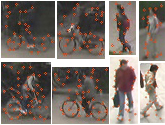
\includegraphics[width=1.0\textwidth,bb=0 0 165 125]{samples.jpg}
\end{minipage}
\label{fig:train:a}
}
\subfigure[]{
{
\begin{minipage}[b]{0.2\textwidth}
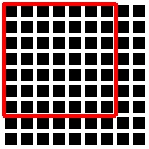
\includegraphics[width=0.3\textwidth,bb=0 0 149 149]{dst6.jpg}
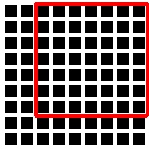
\includegraphics[width=0.3\textwidth,bb=0 0 149 149]{dst3.jpg}
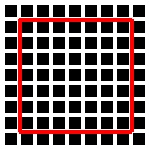
\includegraphics[width=0.3\textwidth,bb=0 0 149 149]{dst5.jpg}  \\
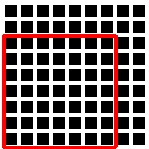
\includegraphics[width=0.3\textwidth,bb=0 0 149 149]{dst2.jpg}
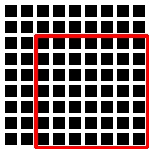
\includegraphics[width=0.3\textwidth,bb=0 0 149 149]{dst4.jpg}
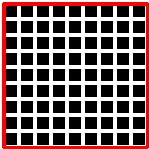
\includegraphics[width=0.3\textwidth,bb=0 0 149 149]{dst1.jpg}
\end{minipage}
}
\label{fig:train:b}
}
\caption{(a) Training images. Note some keypoints fall on the background. (b) The manner how a 9$\times$9 image patch is used to generate six region covariances, and red rectangles indicate the pixels used for each covariance.}
\label{fig:train}
\end{figure}

\textbf{Dataset} 

\textbf{Implementation Settings}


\begin{figure}
\centering
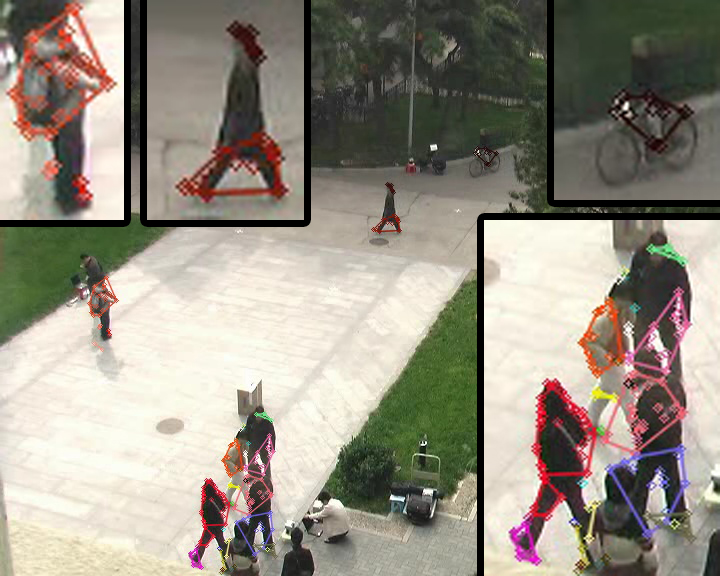
\includegraphics[width=0.23\textwidth,bb=0 0 720 576]{a16.jpg}
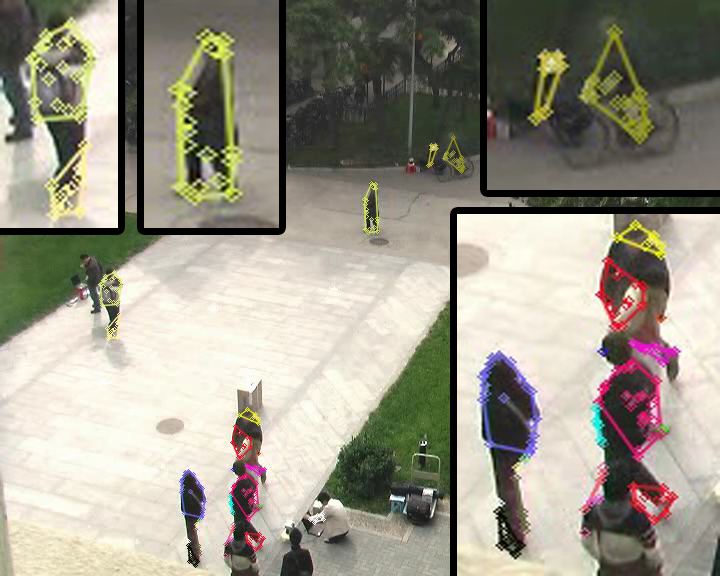
\includegraphics[width=0.23\textwidth,bb=0 0 720 576]{a26.jpg}
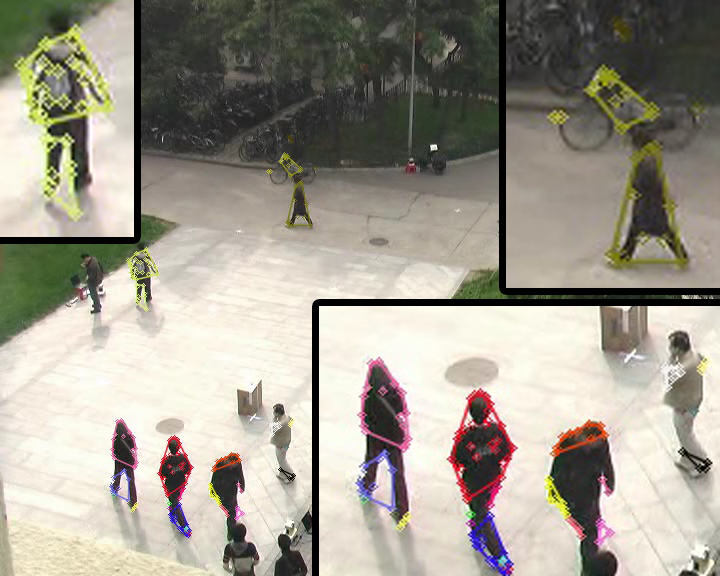
\includegraphics[width=0.23\textwidth,bb=0 0 720 576]{a71.jpg}
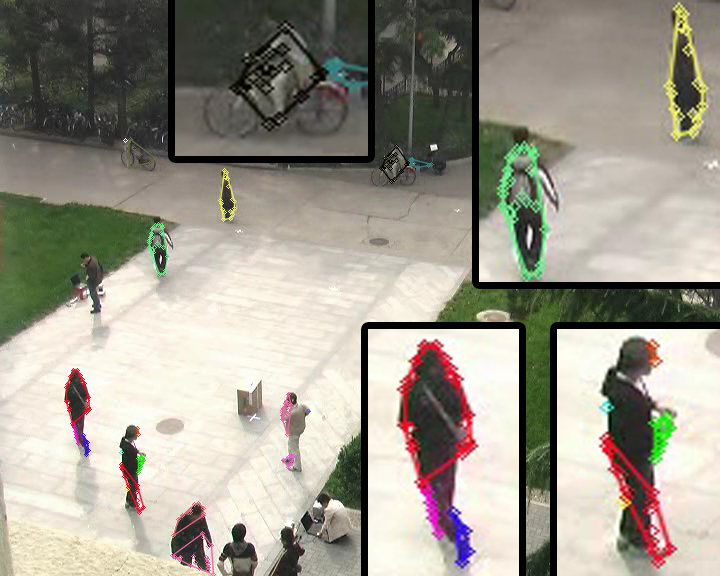
\includegraphics[width=0.23\textwidth,bb=0 0 720 576]{a116.jpg}
\caption{Motion grouping results.}
\label{fig:mgr}
\end{figure}



\textbf{Comparisons} 
\begin{figure}
\centering
\subfigure[]{
\begin{minipage}[b]{0.22\textwidth}
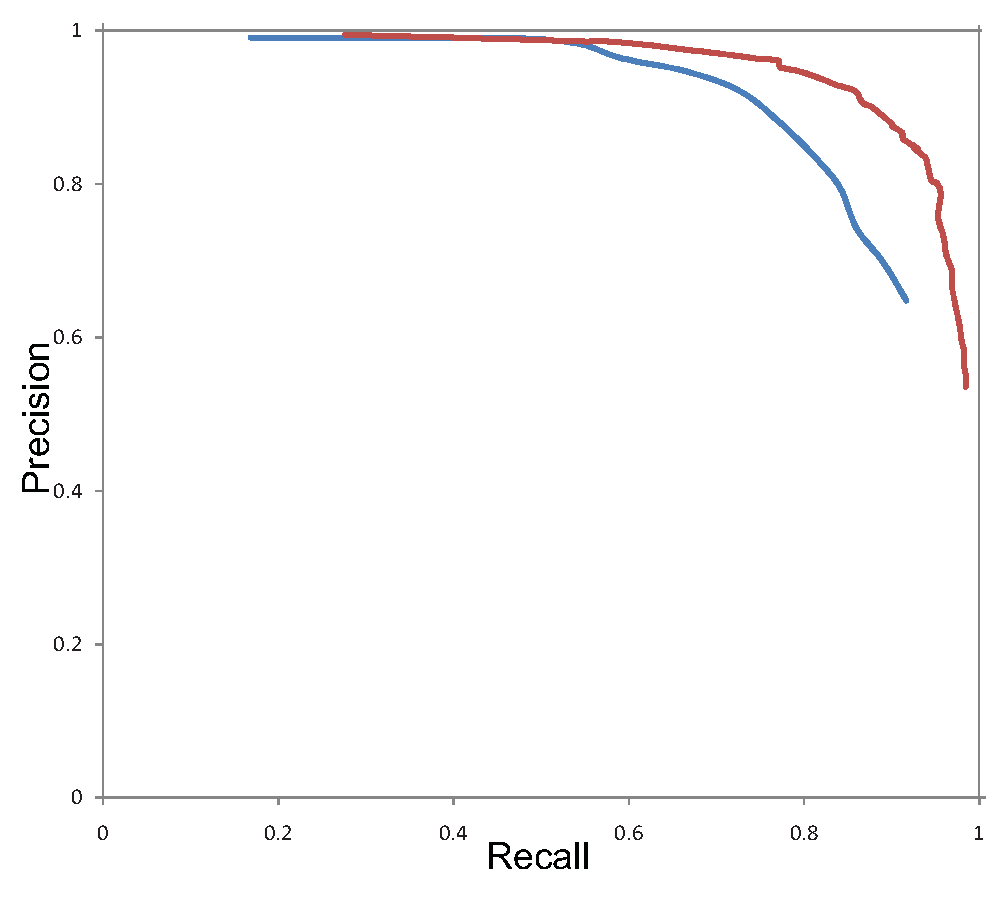
\includegraphics[width=1\textwidth,bb=0 0 480 425]{prf.eps}
\end{minipage}
\label{fig:pr:a}}
\subfigure[]{
\begin{minipage}[b]{0.22\textwidth}
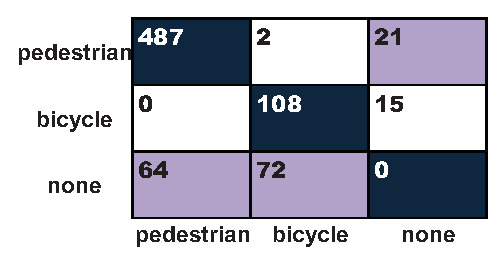
\includegraphics[width=\textwidth,bb=0 0 230 115]{cm2.eps}\\
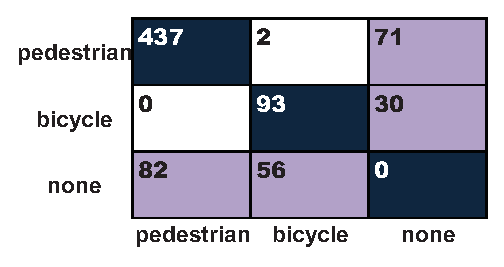
\includegraphics[width=\textwidth,bb=0 0 230 115]{cm1.eps}
\end{minipage}
\label{fig:pr:b}}
\caption{(a) Precision-recall curves (red: the proposed method, blue: the benchmark method). (b) Confusion matrices (upper: the proposed method, lower: the benchmark method).}
\label{fig:pr}
\end{figure}



\begin{figure*}
\centering
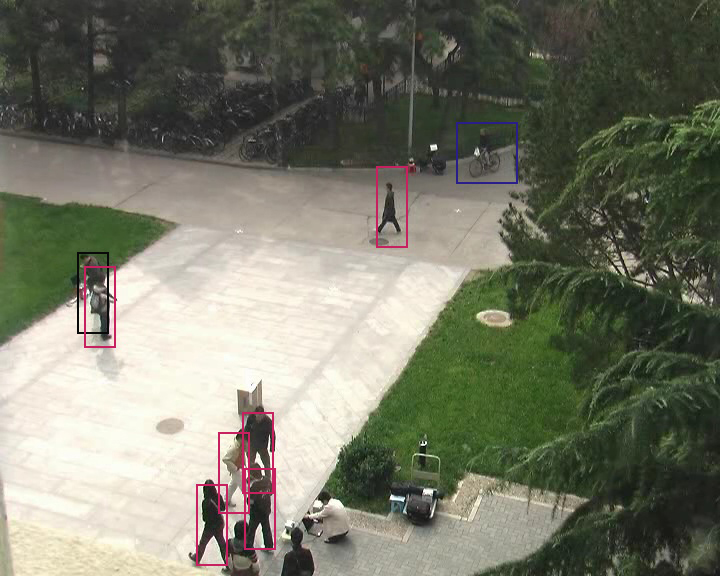
\includegraphics[width=0.23\textwidth,bb=0 0 720 576]{016.jpg}
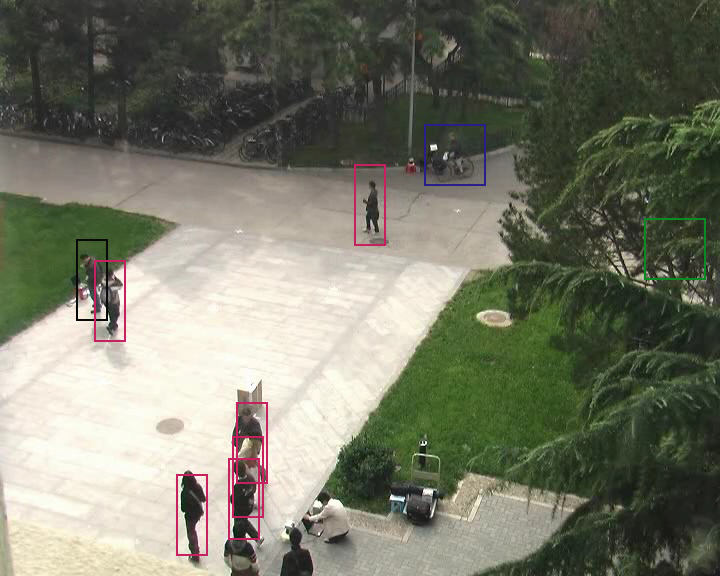
\includegraphics[width=0.23\textwidth,bb=0 0 720 576]{026.jpg}
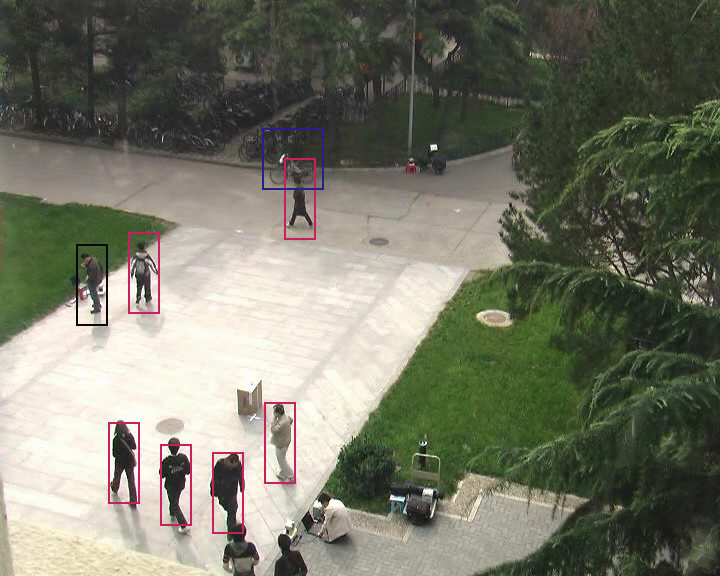
\includegraphics[width=0.23\textwidth,bb=0 0 720 576]{071.jpg}
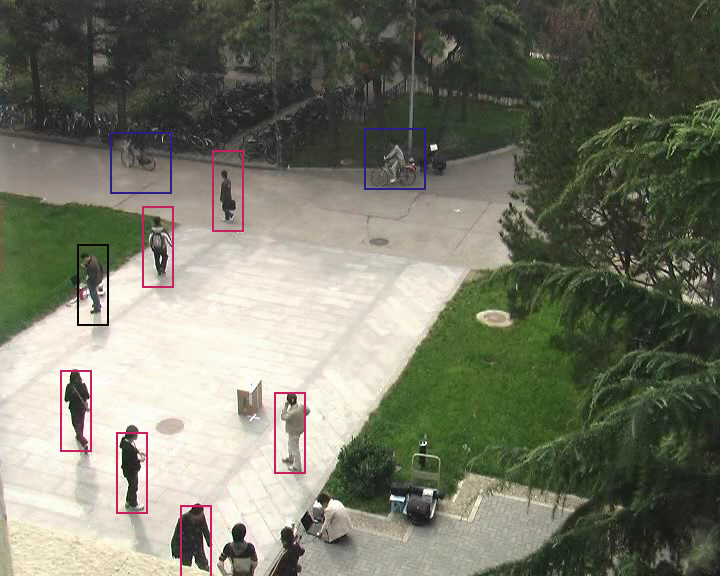
\includegraphics[width=0.23\textwidth,bb=0 0 720 576]{116.jpg}\\
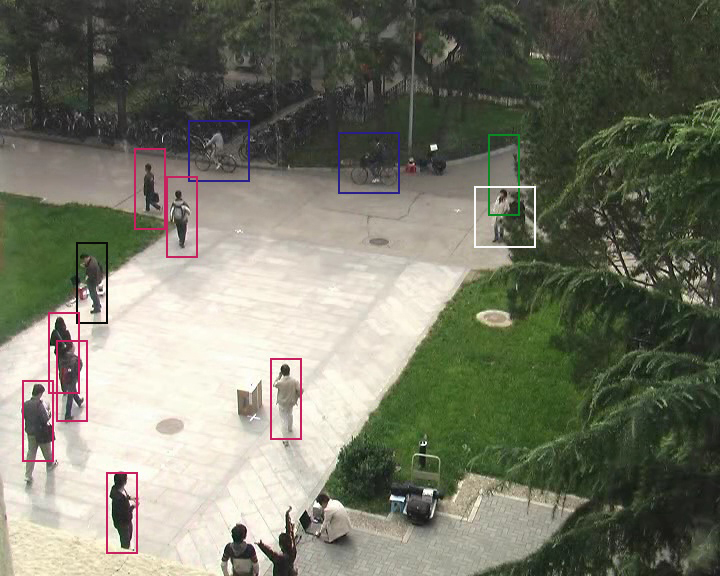
\includegraphics[width=0.23\textwidth,bb=0 0 720 576]{166.jpg}
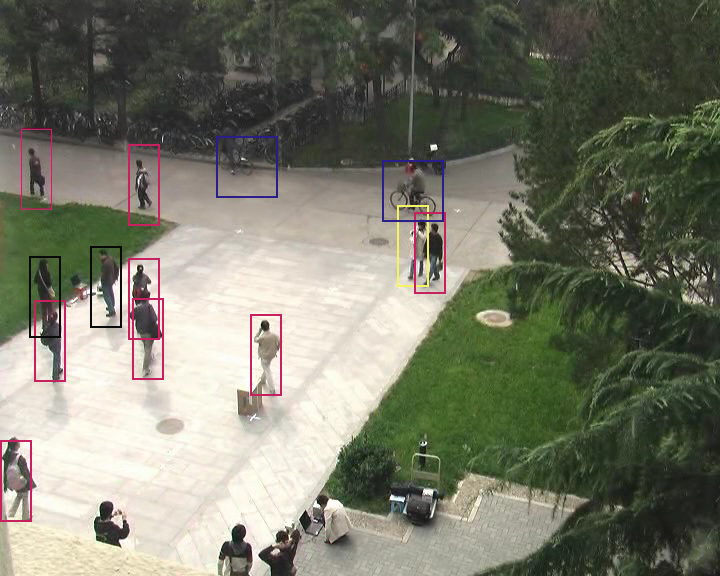
\includegraphics[width=0.23\textwidth,bb=0 0 720 576]{251.jpg}
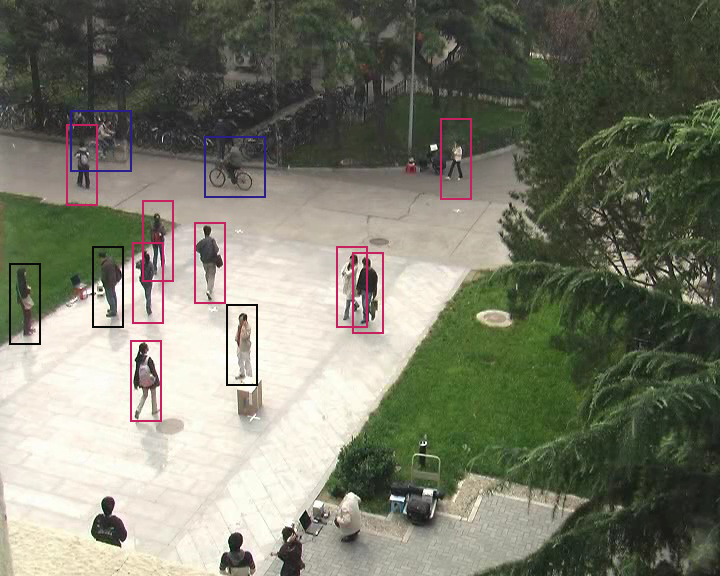
\includegraphics[width=0.23\textwidth,bb=0 0 720 576]{326.jpg}
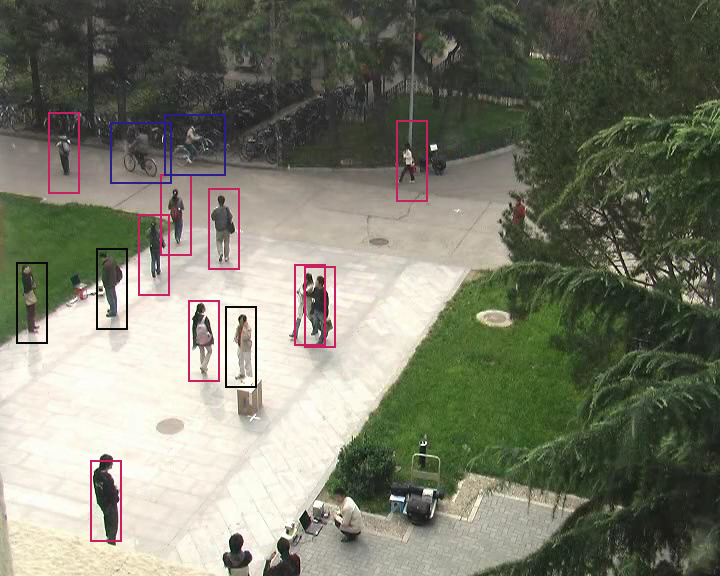
\includegraphics[width=0.23\textwidth,bb=0 0 720 576]{366.jpg}
\caption{Results. Red rectangles and blue rectangles mark correctly detected pedestrians and bicycle riders. Yellow rectangles mark missed detections. White rectangles mark correctly detected but not correctly labeled objects. Green rectangles mark false alarms. Black rectangles mark static objects which are beyond the verification of this method.}
\label{fig:result}
\end{figure*}



\subsection{Wild-scene Detection}

\begin{figure}
\centering
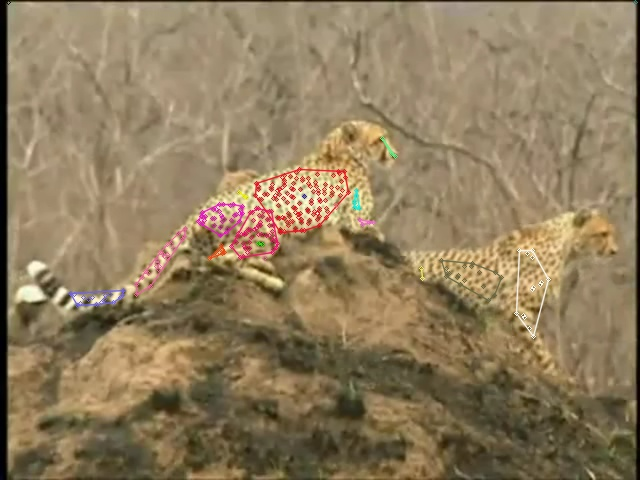
\includegraphics[width=0.23\textwidth,bb=0 0 640 480]{amotionimg00296.jpg}
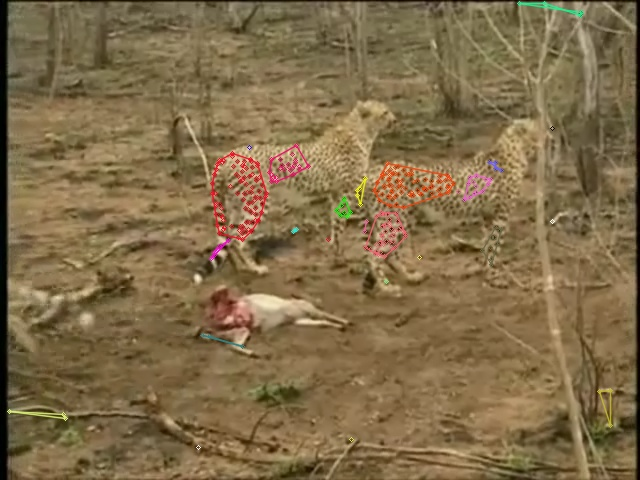
\includegraphics[width=0.23\textwidth,bb=0 0 640 480]{amotionimg01836.jpg}

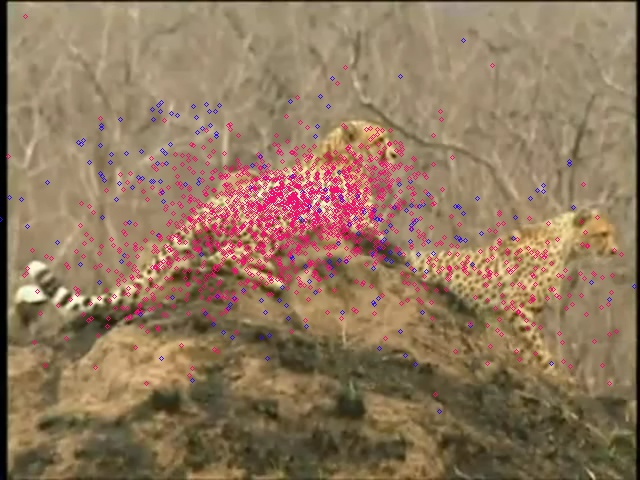
\includegraphics[width=0.23\textwidth,bb=0 0 640 480]{selectVimg00296_0.jpg}
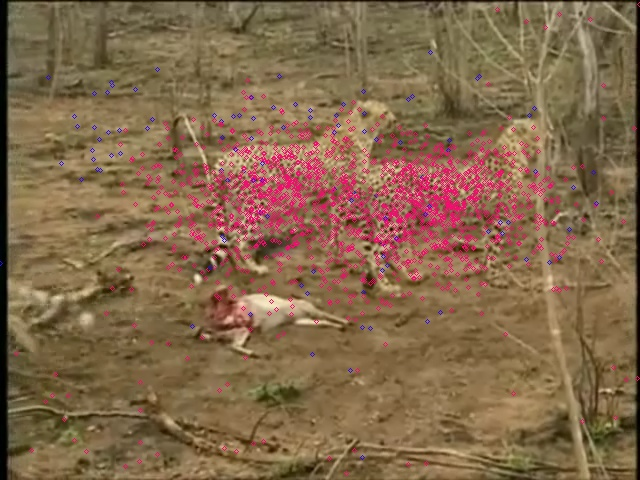
\includegraphics[width=0.23\textwidth,bb=0 0 640 480]{selectVimg01836_0.jpg}

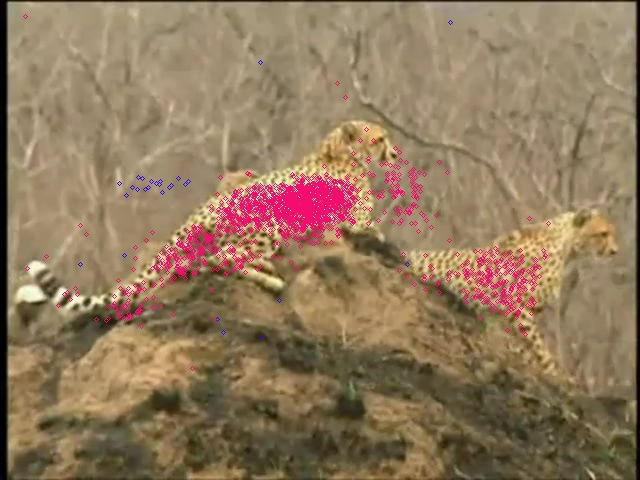
\includegraphics[width=0.23\textwidth,bb=0 0 640 480]{selectVimg00296_19.jpg}
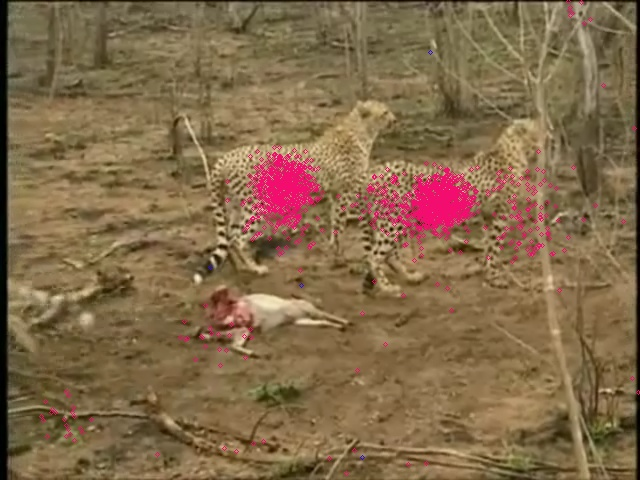
\includegraphics[width=0.23\textwidth,bb=0 0 640 480]{selectVimg01836_19.jpg}

\caption{Effect of the proposed weight assignment. Red circles are voted centers for leopards, while blue ones are voted centers for tigers. On the top are the motion grouping results. In the middle are the voted centers according to the best matched codes. On the bottom are the voted centers voted by votes with the highest weights.}
\label{fig:bcMP}
\end{figure}

\begin{figure}
\centering


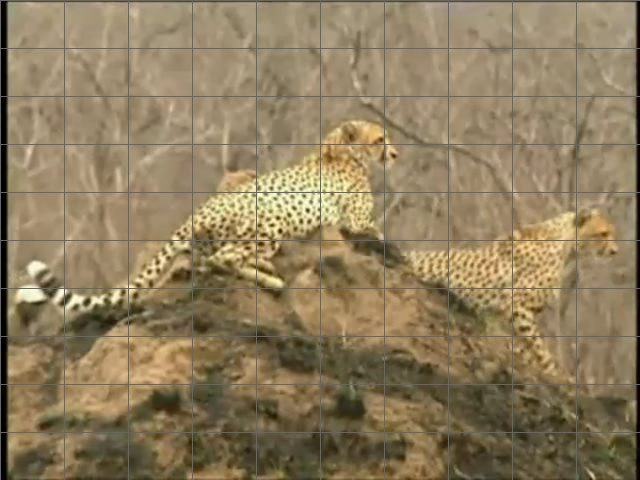
\includegraphics[width=0.23\textwidth,bb=0 0 640 480]{PER1.jpg}
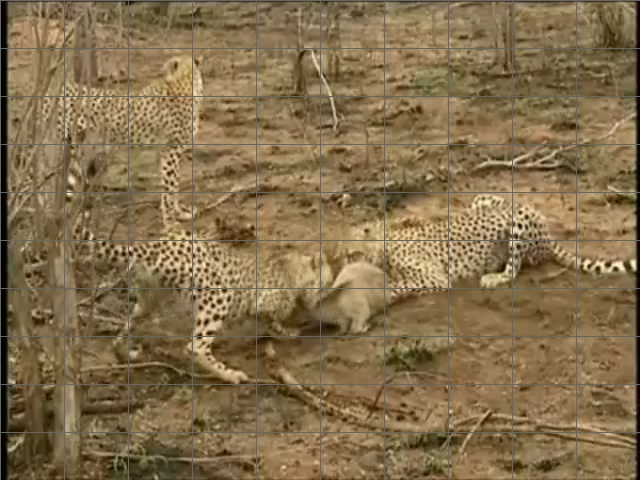
\includegraphics[width=0.23\textwidth,bb=0 0 640 480]{PER2.jpg}

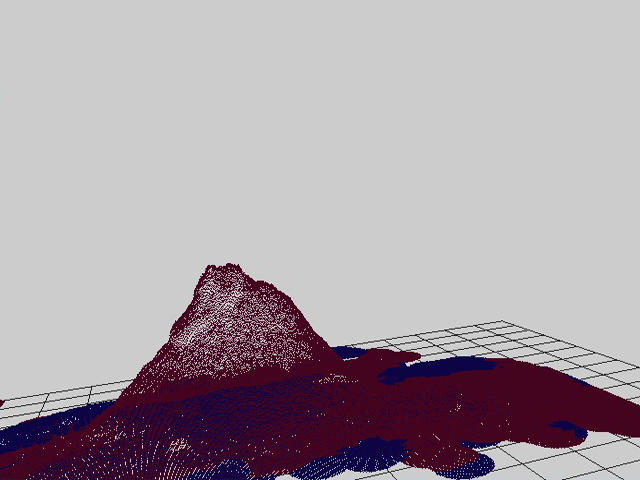
\includegraphics[width=0.23\textwidth,bb=0 0 640 480]{1.jpg}
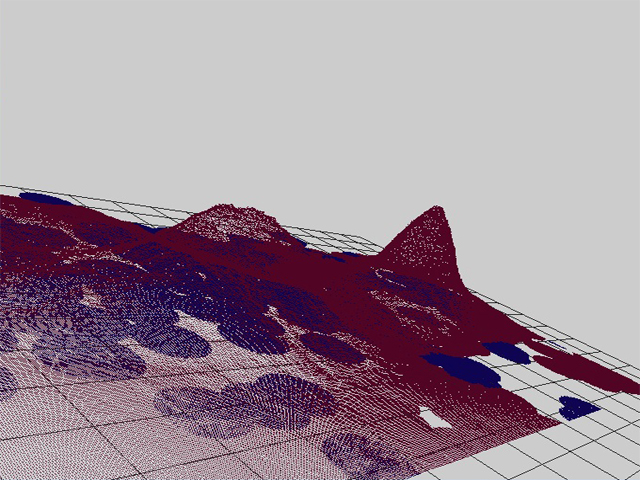
\includegraphics[width=0.23\textwidth,bb=0 0 640 480]{3.jpg}

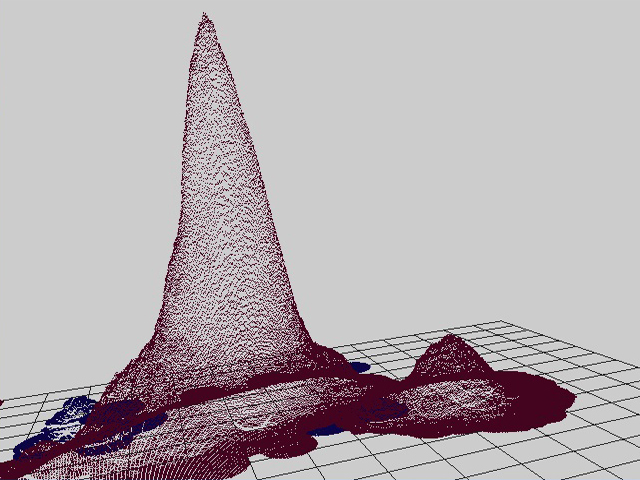
\includegraphics[width=0.23\textwidth,bb=0 0 640 480]{2.jpg}
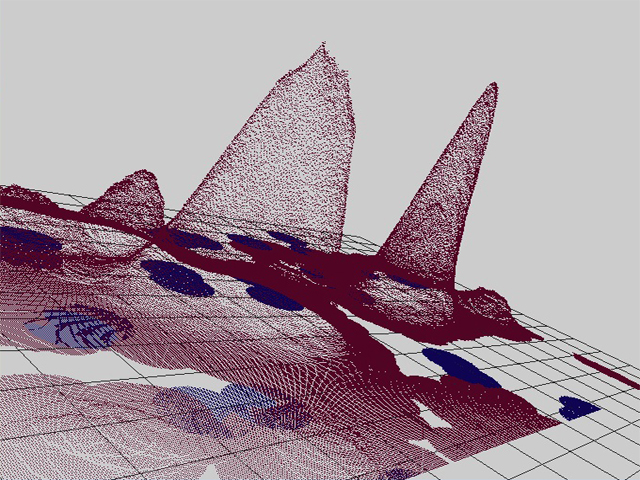
\includegraphics[width=0.23\textwidth,bb=0 0 640 480]{4.jpg}


\caption{Example Hough images. On the top are the original images. In the middle are the Hough images formed by votes with uniform priors. On the bottom are the Hough images formed by votes with the proposed weights. Red indicates leopards, and blue indicates tigers. Note that for the two leopards, there is no peak corresponding to the one on the right, on the benchmark Hough image. For the three leopards, there is also no peak corresponding to the leopard behind on the benchmark Hough image.}
\label{fig:BcHi}
\end{figure}
\textbf{Dataset} 
\textbf{Implementation settings} 




\textbf{Comparisons} 

\begin{figure}
\centering
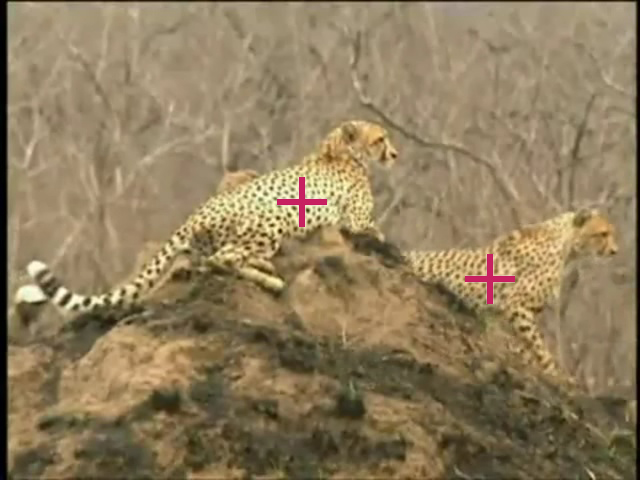
\includegraphics[width=0.23\textwidth,bb=0 0 640 480]{leo1.jpg}
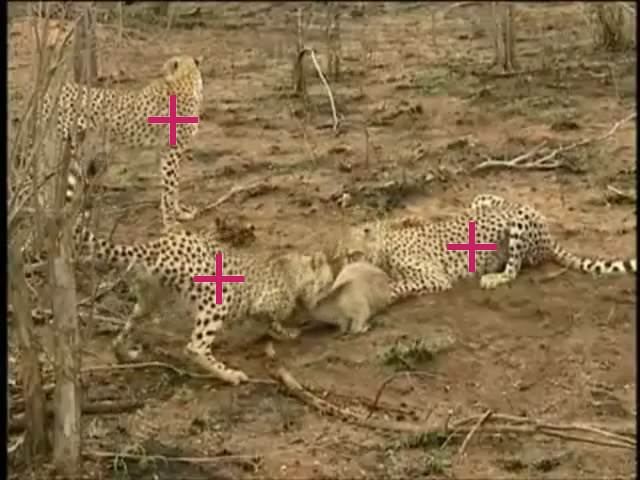
\includegraphics[width=0.23\textwidth,bb=0 0 640 480]{leo2.jpg}

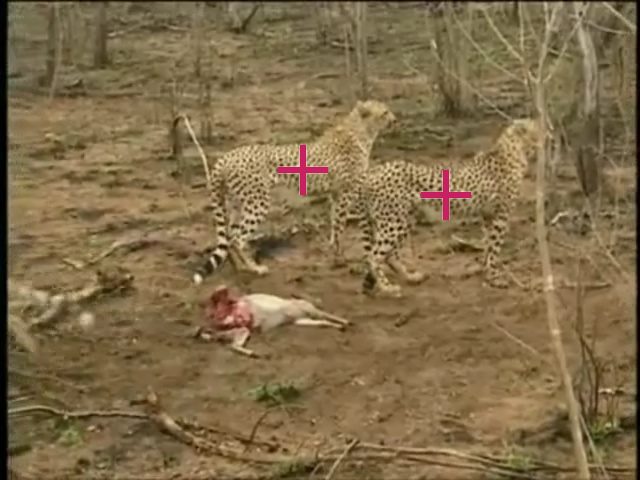
\includegraphics[width=0.23\textwidth,bb=0 0 640 480]{leo3.jpg}
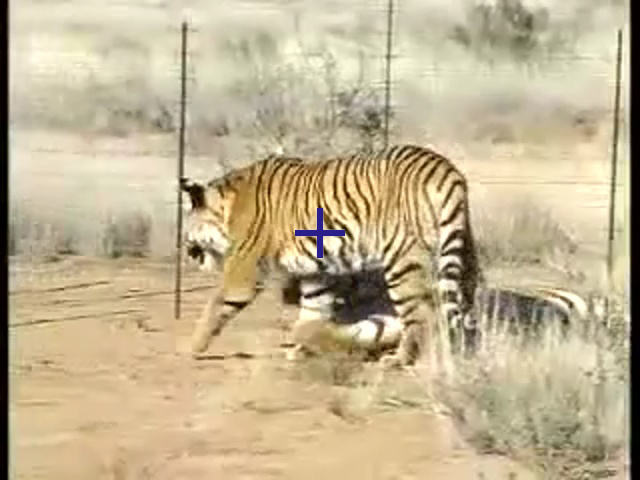
\includegraphics[width=0.23\textwidth,bb=0 0 640 480]{ti1.jpg}

\caption{Results. Red crosses mark the centers for leopards and blue crosses mark the centers for tigers.}
\label{fig:bgdr}
\end{figure}
\section{Conclusion}
The computational ability of human beings is limited, while their ability to detect is far beyond that of machines. Thus, it is very possible that this detection ability benefits from multiple perceptual mechanisms. By using one of these mechanisms, we propose a detection method.  By embedding motion grouping results into the voting schema of hough transforms, the method is able to distinguish near objects' positions, distinguish similar objects' labels, and maintain the detection rate with a noisy codebook. The success of our method further demonstrates the advancement of perceptual mechanisms in human beings. And the success of this method will help with detection methods in ITS areas.
% conference papers do not normally have an appendix


% use section* for acknowledgement
\section*{Acknowledgment}
This work was, in part, supported by SCOPE program by the Ministry of Internal Affairs and Communications. Part of the work was done during the first author's master course at Peking University. The first author is sponsored by China Scholarship Council. The authors thank Bo Zheng, Boxin Shi, Patricia Knapp, and Nicole Hajicek for suggestions.





% trigger a \newpage just before the given reference
% number - used to balance the columns on the last page
% adjust value as needed - may need to be readjusted if
% the document is modified later
%\IEEEtriggeratref{8}
% The "triggered" command can be changed if desired:
%\IEEEtriggercmd{\enlargethispage{-5in}}

% references section

% can use a bibliography generated by BibTeX as a .bbl file
% BibTeX documentation can be easily obtained at:
% http://www.ctan.org/tex-archive/biblio/bibtex/contrib/doc/
% The IEEEtran BibTeX style support page is at:
% http://www.michaelshell.org/tex/ieeetran/bibtex/
%\bibliographystyle{IEEEtran}
% argument is your BibTeX string definitions and bibliography database(s)
%\bibliography{IEEEabrv,../bib/paper}
%
% <OR> manually copy in the resultant .bbl file
% set second argument of \begin to the number of references
% (used to reserve space for the reference number labels box)

{\small
\bibliographystyle{ieee}
\bibliography{egbib}
}
%\renewcommand{\captionlabeldelim}{}
\parpic{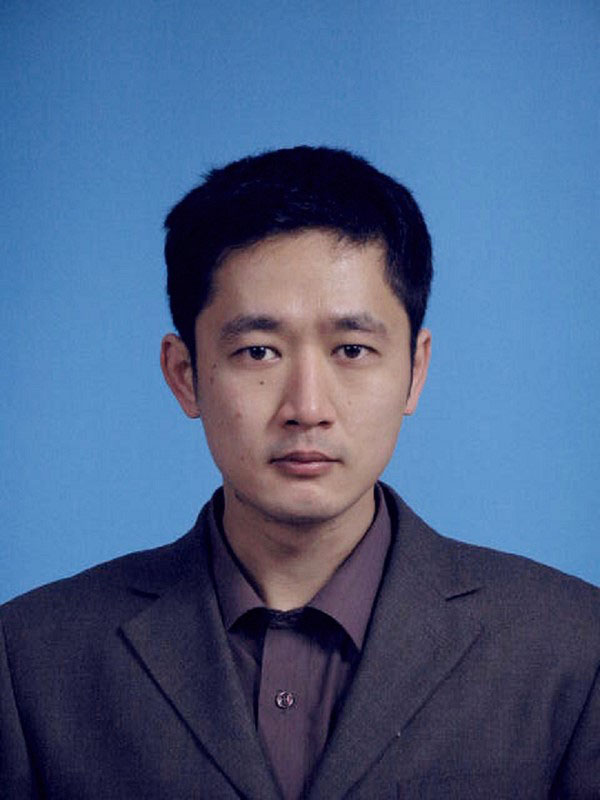
\includegraphics[width=0.13\textwidth,bb=0 0 600 800]{wzp.jpg}}
\noindent {\bf Zhipeng Wang} received his B.S. degree in Industrial Engineering from Tsinghua University, China, in 2007. He received his M.S. degree in Computer Applied Technology
  from Peking University, 2010 and is currently a Ph.D. student in the Department of Computer Science, the University of Tokyo. His research interests are in the areas of computer vision and machine learning.

\parpic{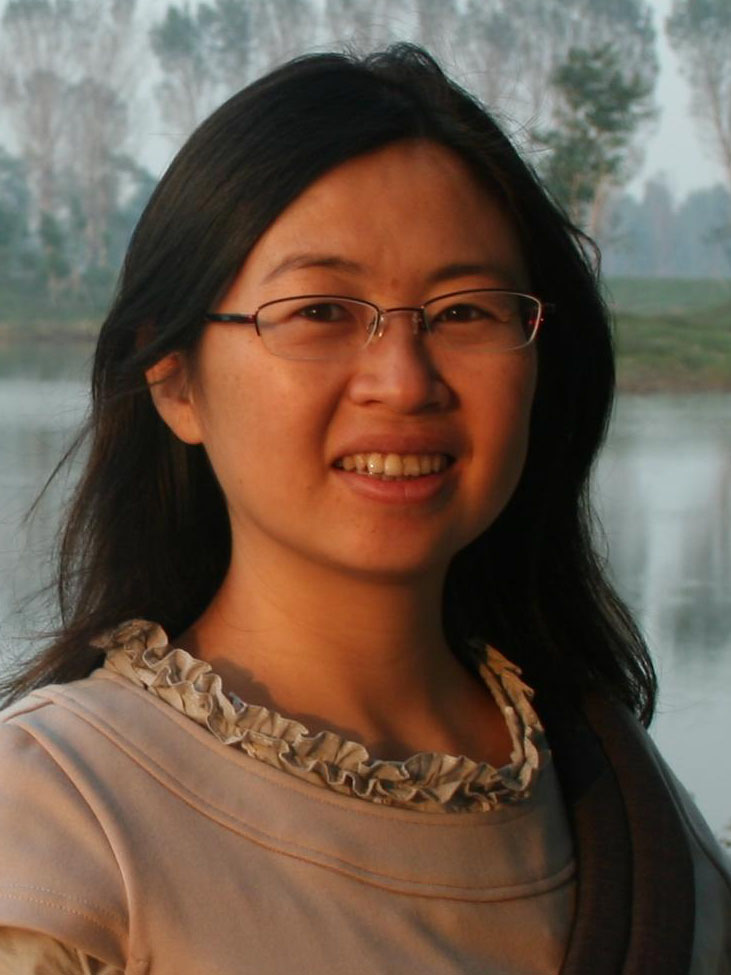
\includegraphics[width=0.13\textwidth,bb=0 0 731 975]{cjs.jpg}}
\noindent {\bf Jinshi Cui}  received the B.S. and Ph.D. degrees
in computer science from Tsinghua University,
Beijing, China, in 1999 and 2004, respectively.
In 2004, she joined the School of Electronics Engineering
and Computer Science, Peking University,
Beijing, as an Assistant Professor. She was promoted
to Associate Professor in 2007. Her research interests
include computer vision and robotics.


\parpic{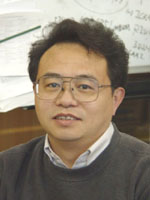
\includegraphics[width=0.13\textwidth,bb=0 0 150 200]{zhb.jpg}}
\noindent {\bf Hongbin Zha} received the B.E. degree in 	
electrical engineering from Hefei University of Tech-	
nology, Hefei, China, in 1983 and the M.S. and 	
Ph.D. degrees in electrical engineering from Kyushu 	
University, Fukuoka, Japan, in 1987 and 1990, 	
respectively. 	
After being a Research Associate with Kyushu 	
Institute of Technology, he joined Kyushu University 	
in 1991 as an Associate Professor. In 1999, he was 	
also a Visiting Professor with the Centre for Vision, 	
Speech, and Signal Processing, Surrey University, 	
Surrey, U.K. Since 2000, he has been a Professor with the Center for Infor-	
mation Science, School of Electronics Engineering and Computer Science, 	
Peking University, Beijing, China. He has published more than 200 technical 	
publications in journals, books, and international conference proceedings. His 	
research interests include computer vision, digital geometry processing, and 	
robotics. 	
Dr. Zha was the recipient of the Franklin V. Taylor Award from the IEEE 	
Systems, Man, and Cybernetics Society in 1999. 	



\parpic{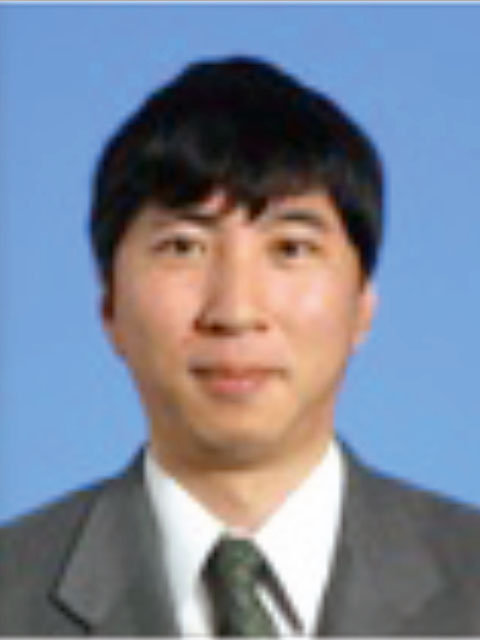
\includegraphics[width=0.13\textwidth,bb=0 0 480 640]{mk.jpg}}
\noindent {\bf Masataka Kagesawa} received the BS degree in mathematics in 1986
from Chiba University, Japan, the MS degree in mathematics
from Tokyo Metropolitan University in 1988.  He was a doctor
course student at Tokyo Metropolitan University from 1988 to
1990.  From 1990 to 1994, he was a technical associate at the
Institute of Industrial Science, the university of Tokyo.
He is now a research associate at the same institute.
He received the PhD degree in electronic engineering in 2003 from the
university of Tokyo.
His research
interests include traffic simulation with dynamic information,
traffic management systems and sensing systems on Intelligent
Road Traffic Systems.

\parpic{\includegraphics[width=0.13\textwidth,bb=0 0 120 160]{os.jpg}}
\noindent {\bf Shintaro Ono}  received the BE degree in 2001 and PhD degree in 2006 from The University of Tokyo.
Currently he is a Project Associate Professor in Advanced Mobility Research Center (ITS Center), The University of Tokyo.
His research interests include sensing system and computer vision/graphics for ITS, and digital archiving of cultural heritage objects.


\parpic{\includegraphics[width=0.13\textwidth,bb=0 0 354 472]{ki.jpg}}
\noindent {\bf Katsushi Ikeuchi}  is a Professor at the Institute of Industrial Science, the��University of Tokyo, Tokyo, Japan. He received the Ph.D. degree in��Information Engineering from the University of Tokyo, Tokyo, Japan, in 1978.��After working at the Artificial Intelligence Laboratory, MIT for three��years, the Electrotechnical Laboratory, MITI for five years, and the School��of Computer Science, Carnegie Mellon University for ten years, he joined the��university in 1996.

He has served (or will serve) as the program/general chairman of several��international conferences, including 1995 IEEE-IROS (General), 1996��IEEE-CVPR (Program), 1999 IEEE-ITSC (General) and 2003 ICCV (Program). He is an Editor-in-Chief of the International Journal of Computer Vision. He has been a fellow of IEEE since 1998. He was selected as a distinguished lecture of IEEE SP society for the period of 2000-2001.

He has received several awards, including the David Marr Prize in computational vision, IEEE RA society K-S Fu memorial best transaction paper award, Computer Vision Significant Researcher Award, and Medal with Purple Ribbon. In addition, in 1992, his paper, "Numerical Shape from Shading and Occluding Boundaries," was selected as one of the most influential papers to have appeared in Artificial Intelligence Journal within the past ten years.


\end{document}
